% !TEX root = ../Report.tex
\subsection{DeepMedic architecture}
DeepMedic is a 3D Neural Network. It has been initially used for segmentations in biomedical 3D scans, especially for detecting brain anomalies such as injuries, tumors and lesions. In this project we have been able to try this algorithm on lung segmentations. \newline 
A DeepMedic model consists of detecting a particular pattern in an image. This is achieved by convolution  at  following layers of the network. We distinguish two components in the model. First there is a three-dimension Convolutional Neural Network (CNN) model used for dense segmentation, then  a three-dimension fully connected conditional random field (CRF) model for deeper predictions. (Might we only use the first component?) \newline
Each layer of the CNN model contains channels called feature maps, i.e. a group of neurons identifying a feature in the previous layer. Then a feature is defined by associated kernel weights. Number of inputs, outputs, feature-maps and kernels are tunable.


\iffalse 
\begin{figure}[h]
	\includegraphics{files/deepmedic.png}
	\caption{\label{deepmedic} Overview of DeepMedic architecture}
\end{figure}
\fi

\subsection{U-Net architecture}
Semantic segmentation is partition of an image in coherent parts. For end to end encoding decoding network unet is used for semantic segmentation. Unet is mostly used for biomedical image segmentation. The following image shows how unet works.\newline

\begin{figure}[h!]
	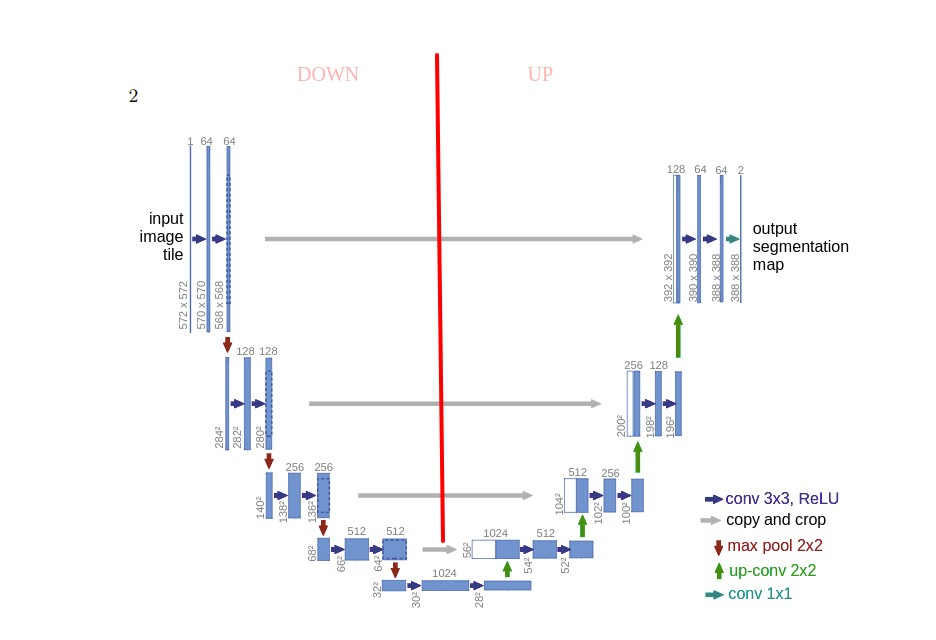
\includegraphics[width=0.49\textwidth, angle=0]{files/unetstructure.jpg}
	\caption{CT scan of the lung and labeled parts}
	\label{unetstructure}
\end{figure}

This is a U-net architecture . Each bluebox corresponds to a multi-channel feature map. The number of channels is denoted on top of the box. The x-y-size is provided at the lower left edge of the box. White boxes represent copied feature maps. The arrows denote the different operations.\newline
The first part is called down or encoder part where we will apply convolutional blocks followed by maxpool downsampling to encode the input image into feature representations at multiple different levels. The second part of the network consists of upsample and concatenation followed by regular convolution operations. We are going to expand the future dimensions from left to meet the same size  with concatenation blocks. The grey and green arrows tell from where to concatenate future maps together. The main feature of unet in comaprison to other fully convolutional segmentation networks is that while upsampling and going deeper in the networks we are concatinating the higher resolution features from downpart with upsampled features in order to better localize and learn representation with upcoming convolutions. As upsampling is sparse we need to be good prior from beginning stages to get the better localization representation. In order to get consistent size we applied padded convolutions to keep dimensions consistent across concatination. Localization is one of the most important feature in case of biomedicalimage processing. In order to localize, high resolution from the contracting path are combined with upsampled output. By this the successive convolution layer can then learn to assemble a more precise output. The main modification in our architecture was that in the upsampling part we have a large number of feature channels, which allows the network to propogate context information to high resolution layers. To predict the pixels in the border region of the image, the missing context is extrapolated by mirroring the input image.
